\documentclass[12pt,a4paper]{article}
\usepackage[utf8]{inputenc}
\usepackage[german]{babel}
\usepackage[T1]{fontenc}
\usepackage{amsmath}
\usepackage{amsfonts}
\usepackage{amssymb}
\usepackage{graphicx}
\usepackage{siunitx}
\usepackage[left=2cm,right=2cm,top=2cm,bottom=2cm]{geometry}
\author{Tim}

\begin{document}
\setlength{\parindent}{0pt} 
\begin{center}
{\LARGE Versuchsprotokoll}\\
\begin{large}
zum Grundpraktikum Physik Teil II\\[0.4cm]
an der RWTH Aachen\\
I. Physikalisches Institut B\\[4.5cm]
\Large\textbf{\textsl{Optik II}}\\[4cm]
\normalsize\textit{vorgelegt\\von}\\[0.4cm]
\large{Moritz Berger\\Tim Herbermann\\Gerald Kolter\\Sebastian Siebert}\\[1cm]
\large \textit{Gruppe A07} \\ [3cm]
\large \textbf{Sommersemester 2017}
\end{large}
\end{center}
\newpage

\tableofcontents
\newpage

\section{Grundlagen}

\subsection{Versuchsbeschreibung}
Im folgenden Versuch soll mithilfe eines Michelson-Interferometers die Wellenlänge eines Lasers bestimmt werden. Anschließend soll die Druckabhängigkeit des Brechungsindex von Luft untersucht werden. Im dritten Teilversuch wird der Brechungsindex von $\text{CO}_2$ bestimmt.\\

\subsection{Physikalische Grundlagen}

\paragraph{Michelson-Interferometer}\mbox{}\\
Grundlage des Versuches ist  die Interferenz eines kohärenten Wellenzuges mit sich selbst durch Amplitudenaufspaltung. Die dadurch entstehenden Teilstrahlen durchlaufen unterschiedliche optische Weglängen und werden anschließend wieder vereinigt. Dadurch besitzen sie eine feste Phasenbeziehung zueinander,  sind also kohärent und damit interferenzfähig.\\
Beim Michelson-Interferometer kommt es aufgrund einer gewissen Strahldivergenz zur Ausbildung von Interferenzringen durch den zusätzlichen Wegunterschied. Für die Phasendifferenz ergibt sich dann der Zusammenhang:
 
\begin{equation}
\delta = \dfrac{2\pi}{\lambda} \cdot 2d \cos(\theta)
\end{equation}

Betrachtet man Interferenzmaxima muss $\delta = 2\pi m$, $m=0,1,2,...$, gelten und damit

\begin{equation}
2d \cos(\theta) = m\lambda
\label{equ:Maxima}
\end{equation}

für die Beschreibung der Interferenzringe.

\paragraph{Brechungsindex}\mbox{}\\
Der Brechungsindex eines Gases hängt im allgemeinen von seinem Druck ab.\\
Durch Taylorentwicklung ergibt sich als lineare Näherung für die Druckabhängigkeit des Brechungsindexes die Formel:

\begin{equation}
n(P) = 1+\frac{\Delta n}{\Delta P} \cdot P
\label{eq:DruckBrechzahl}
\end{equation}

Aus der optischen Wegdifferenz bei Veränderung des Brechungsindex und der Maximumsbedingung ergibt sich für das Zentrum des Schirms (d.h. $\theta = 0$) der Zusammenhang:

\begin{equation}
\frac{\Delta n}{\Delta P} = \frac{\Delta m}{\Delta P} \cdot  \frac{\lambda}{2L}
\label{equ:DruckBrechung}
\end{equation}

Ähnliche Überlegungen bezüglich der optischen Wegdifferenz für den Brechungsindex von $\text{CO}_2$ führen zu den Zusammenhängen:

\begin{equation}
n_{CO_2} = n_{Luft} + \Delta n
\label{eq:COO_n}
\end{equation}


\begin{equation}
\Delta n = \Delta m \frac{\lambda}{2L}
\label{eq:COO_dn}
\end{equation}



\section{Aufbau und Durchführung}

\subsection{Aufbau}
\begin{figure}
\centering
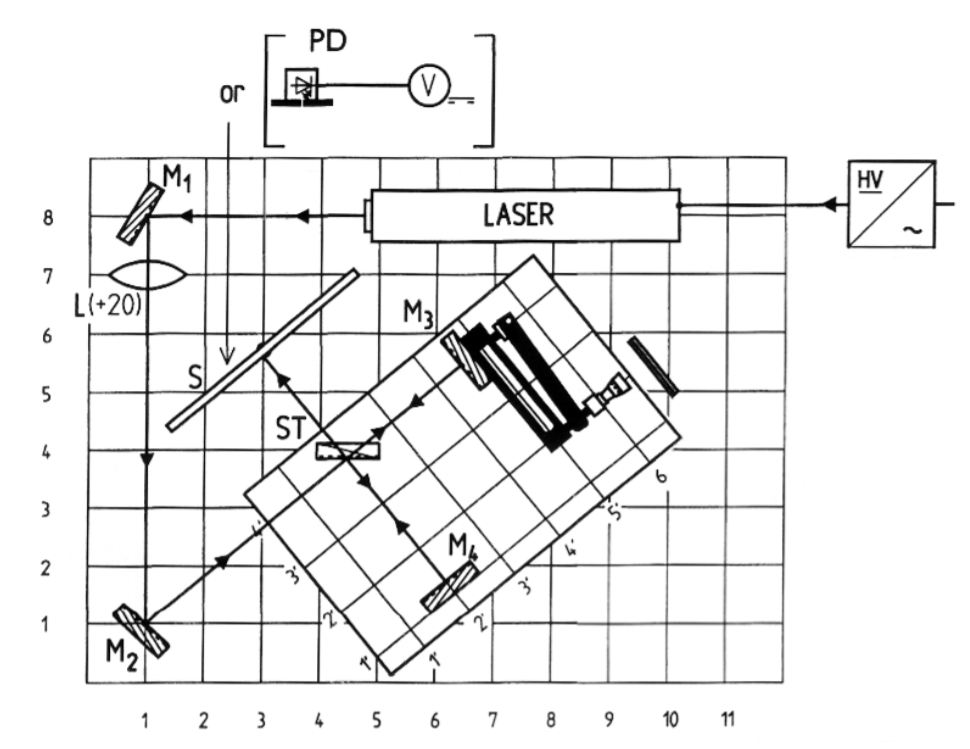
\includegraphics[scale=0.6]{Bilder/Aufbau}
\caption{Aufbau eines Michelson-Interferometers. (Quelle: Praktikumsskript S.37)}
\label{fig:Aufbau}
\end{figure}

\begin{figure}
\begin{center}
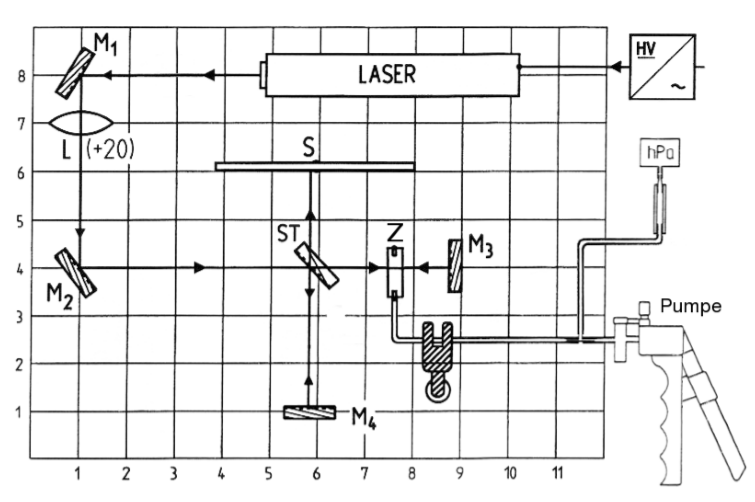
\includegraphics[scale=0.6]{Bilder/AufbauDruck.png}
\caption{Aufbau zur Bestimmung der Druckabhängigkeit des Brechungsindex. (Quelle: Praktikumsskript S.41)}
\label{fig:AufbauDruck}
\end{center}
\end{figure}

Der Aufbau besteht im wesentlichen aus einem Michelson-Interferometer. Über die Spiegel M1 und M2 wird der Laserstrahl auf den Strahlteiler gelenkt, wobei zusätzlich eine Linse zur Strahlaufweitung durchlaufen wird. Die geteilten Strahlen werden am Spiegel M4 und am verstellbaren Spiegel M3 reflektiert. Nach erneuter Vereinigung der Strahlen treffen diese Auf dem Schirm S auf. Eine Darstellung des Aufbaus für die Wellenlängenbestimmung ist in Abbildung \ref{fig:Aufbau} gezeigt. Der Versuchsaufbau zur Druckabhängigkeit und zum $\text{CO}_2$ findet sich in Abbildung \ref{fig:AufbauDruck} und unterscheidet sich dadurch, dass im Strahlengang zwischen Strahlteiler und Spiegel M3 zusätzlich eine Glasparzelle eingefügt wird.

\subsection{Durchführung}


Zu Beginn wird die Wellenlänge des grünen Lasers durch Veränderung der optischen Weglänge bestimmt.
Dazu wird der Spiegel M3 (vgl. Abbildung \ref{fig:Aufbau})verschoben, wobei im Interferenzbild am Schirm aufgrund der Veränderung der optischen Weglänge nacheinander im Zentrum Maxima verschwinden bzw. erscheinen. Eine Wechsel von $\Delta m$ Maxima entspricht dann einer gewissen Verschiebung $\Delta d$. Die Wellenlänge des Lasers ergibt sich dann aus Gleichung \ref{equ:Maxima} für $\theta = 0$.\\

Die Verschiebung von M3 erfolgt über einen Feintrieb. Es muss somit zuvor eine Kalibrierung zwischen (relativer) Spiegelposition $d$ und Feintriebskala $s$ vorgenommen werden. Dafür wird ein roter He-Ne-Laser mit bekannter Wellenlänge ($\lambda = 632,8$ nm) verwendet.\\


Die Bestimmung der Druckabhängigkeit findet mit dem modifizierten Aufbau \ref{fig:AufbauDruck} statt. Mit der Handpumpe wird der Druck in der Parzelle solange verringert, bis auf dem Schirm ein vollständiger Wechsel von Maximum zu Maximum durchlaufen wurde. Für jeden dieser Schritte wird der Druck gemessen und notiert. Die Druckabhängigkeit ergibt sich dann durch entsprechende Auftragung mithilfe von Gleichung \ref{equ:DruckBrechung}.

Für die Bestimmung des Brechungsindex von $\text{CO}_2$ wird ebenfalls die Glasparzelle verwendet. Die eingeschlossene Luft wird langsam durch $\text{CO}_2$ ersetzt bis das Volumen vollständig von diesem ausgefüllt wird. Die dabei durchlaufenen Interferenzmaxima werden gezählt. Der Brechungsindex ergibt sich dann durch die Gleichungen \ref{eq:COO_n} und \ref{eq:COO_dn}, wobei $n_{Luft}$ über den zuvor bestimmten Zusammenhang aus dem Umgebungsdruck ermittelt werden muss.

\section{Auswertung}

\subsection{Kalibration}

\subsection{Bestimmung der Wellenlänge}

\subsection{Druckabhängigkeit des Brechungsindex von Luft}

\begin{table}
\begin{center}
\begin{tabular}{|c|c|c|c|c|c|c|}
\hline 
m [1] & $P_1$ [hPa] & $P_2$ [hPa] & $P_3$ [hPa] & $P_4$ [hPa] & $P_5$ [hPa] & $P_6$ [hPa] \\ 
\hline 
0 & 974 & 976 & 977 & 976 & 978 & 976 \\ 
\hline 
1 & 862 & 856 & 865 & 871 & 871 & 846 \\ 
\hline 
2 & 770 & 775 & 773 & 773 & 773 & 766 \\ 
\hline 
3 & 678 & 675 & 674 & 680 & 663 & 655 \\ 
\hline 
4 & 571 & 574 & 570 & 577 & 564 & 544 \\ 
\hline 
5 & 469 & 473 & 467 & 476 & 463 & 457 \\ 
\hline 
6 & 385 & 380 & 369 & 381 & 366 & 363 \\ 
\hline 
7 & 277 & 278 & 269 & 278 & 267 & 260 \\ 
\hline 
8 & 170 & 173 & 161 & 172 & 157 & 160 \\ 
\hline 
9 & 75 & 83 & 66 & 76 & 56 & 69 \\ 
\hline 
\end{tabular} 
\caption{Rohdaten zur Bestimmung der Druckabhängigkeit des Brechungsindexes Aufbau A}
\label{tab:Rohdaten_Druck_A}
\end{center}
\end{table}

\begin{table}
\begin{center}
\begin{tabular}{|c|c|c|c|c|c|c|c|c|}
\hline 
m [1] & $P_1$ [hPa] & $P_2$ [hPa] & $P_3$ [hPa] & $P_4$ [hPa] & $P_5$ [hPa] & $P_6$ [hPa] & $P_7$ [hPa] & $P_8$ [hPa] \\ 
\hline 
0 & 976 & 976 & 976 & 976 & 976 & 976 & 976 & 976 \\ 
\hline 
1 & 866 & 870 & 867 & 858 & 876 & 870 & 882 & 858 \\ 
\hline 
2 & 756 & 763 & 758 & 753 & 773 & 758 & 766 & 753 \\ 
\hline 
3 & 664 & 653 & 668 & 640 & 681 & 667 & 664 & 662 \\ 
\hline 
4 & 541 & 551 & 552 & 525 & 574 & 586 & 562 & 559 \\ 
\hline 
5 & 438 & 455 & 452 & 414 & 480 & 449 & 479 & 457 \\ 
\hline 
6 & 343 & 354 & 348 & 320 & 390 & 368 & - & 352 \\ 
\hline 
7 & - & 252 & 257 & 215 & 269 & 243 & 276 & 264 \\ 
\hline 
8 & - & 154 & 149 & - & 174 & - & 161 & 157 \\ 
\hline 
\end{tabular} 
\caption{Rohdaten zur Bestimmung der Druckabhängigkeit des Brechungsindexes Aufbau B}
\label{tab:Rohdaten_Druck_B}
\end{center}
\end{table}

Der Versuch zur Bestimmung der Druckabhängigkeit des Brechungsindexes wurde an zwei Aufbauten von zwei verschiedenen Experimentatorzweiergruppen durchgeführt. Zur Unterscheidung werden im Folgenden die Bezeichnungen 'Aufbau A' und 'Aufbau B' verwendet.\\
Die Rohdaten von Aufbau A sind in Tabelle \ref{tab:Rohdaten_Druck_A} aufgeführt.\\
Die Rohdaten von Aufbau B sind in Tabelle \ref{tab:Rohdaten_Druck_B} aufgeführt.\\
Zur Auswertung der Daten gibt es zwei Möglichkeiten:
\begin{enumerate}
\item Man verschiebt die Messreihen anhand eines Messpunktes aufeinander und verwendet die Streuung der Punkte für jedes Maximum als Fehler und führt anschließend daran eine lineare Regression durch. 
\item Man führt für alle Messreihen einzeln eine lineare Regression durch und mittelt anschließend die Steigungen. Für diese Variante muss ein Fehler auf die Druckmessung geschätzt werden.
\end{enumerate}
Die Messdaten von Aufbau B eignen sich augenscheinlich besser für Variante 1 als die Messdaten von Aufbau A, da hier bereits der erste Punkt aller Messreihen aufeinander liegen. Die lineare Regression ist in Abbildung \ref{fig:Druck_B_Var1} gezeigt. \\
An den Residuen wird schnell ersichtlich, dass die Fehler deutlich zu groß sind. Dies konnte auch schon an den Messdaten selber erahnt werden, da diese sehr stark streuen.\\
Aus der Steigung kann mittels 
\begin{equation}
\dfrac{dn}{dP} = \dfrac{1}{-a} \cdot \dfrac{\lambda}{2 \cdot l}
\label{equ:Druck_Steigung}
\end{equation}
der Zusammenhang zwischen dem Brechungsindex der Luft und dem Luftdruck bestimmt werden. Der Fehler auf diesen Wert berechnet sich mit dem Fehler auf die Steigung $\sigma _a$ wie folgt bestimmt werden:
\begin{equation}
\sigma _{\frac{dn}{dP}} = \dfrac{dn}{dP} \cdot \sqrt{\left( \dfrac{\sigma_ a}{a} \right) ^2}
\label{equ:Druck_Steigung_Fehler}
\end{equation}
Der Fehler auf die Wellenlänge wird als systematischer Fehler auf das Endergebnis betrachtet. Damit berechnet sich der systematische Fehler zu:
\begin{equation}
\sigma _{\frac{dn}{dP}, sys} = \dfrac{dn}{dP} \cdot \sqrt{\left( \dfrac{\sigma_ \lambda}{\lambda} \right) ^2}
\label{equ:Druck_Steigung_Fehler_sys}
\end{equation}
Unter Verwendung von Gl. \ref{equ:Druck_Steigung}, Gl. \ref{equ:Druck_Steigung_Fehler} und Gl. \ref{equ:Druck_Steigung_Fehler_sys} berechnet sich der Wert für $\dfrac{dn}{dP}$ aus den Daten von Aufbau B nach Methode 1 zu:
\begin{equation*}
\dfrac{dn}{dP} = (2.5931 \pm 0.034 (stat) \pm 0.014 (sys)) \cdot 10^{-7} \, \si{1/mbar}
\end{equation*}

\begin{figure}
\centering
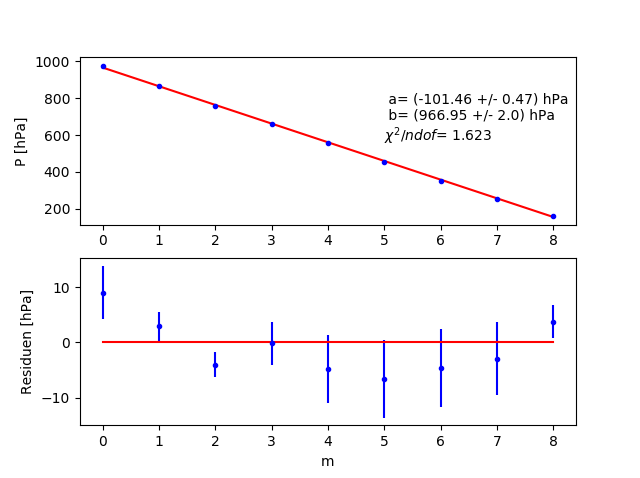
\includegraphics[scale=0.8]{Bilder/Druck_B_Var1.png}
\caption{Lineare Regression nach Variante 1 an Messdaten von Aufbau B.}
\label{fig:Druck_B_Var1}
\end{figure}

\begin{figure}
\centering
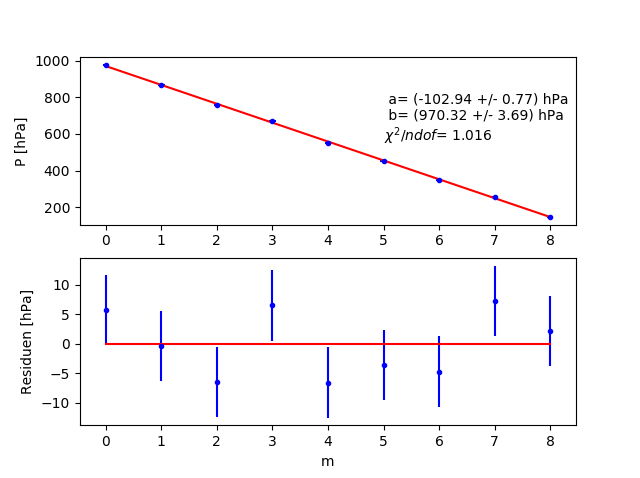
\includegraphics[scale=0.8]{Bilder/Druck_B_Var2.png}
\caption{Lineare Regression beispielhaft an einer Messreihe von Aufbau B.}
\label{fig:Druck_B_Var2}
\end{figure}

\begin{figure}
\centering
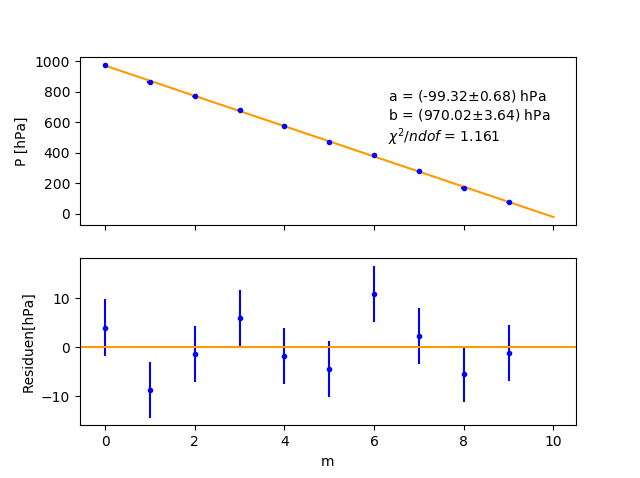
\includegraphics[scale=0.8]{Bilder/Druck_A_Var2_1.png}
\caption{Lineare Regression beispielhaft an einer Messreihe von Aufbau A.}
\label{fig:Druck_A_Var2}
\end{figure}

Abbildung \ref{fig:Druck_B_Var2} zeigt beispielhaft eine der linearen Regressionen an einer der Messreihen von Aufbau B, die der Auswertung nach Variante 1 dienen. Abbildung \ref{fig:Druck_A_Var2} zeigt dies für Aufbau A. \\
Die aus den verschiedenen Messreihen ermittelten Steigungen für diese linearen Regressionen sind für Aufbau B in Tabelle \ref{tab:Druck_Steigungen_B} aufgeführt. Tabelle \ref{tab:Druck_Steigungen_A} zeigt die Steigungen für Aufbau A.

\begin{table}
\begin{center}
\begin{tabular}{|c|c|c|}
\hline 
Messreihe & a & $\sigma _a$ \\ 
\hline 
1 & -106.15 & 1.31 \\ 
\hline 
2 & -102.67 & 0.73 \\ 
\hline 
3 & -102.94 & 0.77 \\ 
\hline 
4 & -108.99 & 1.15 \\ 
\hline 
5 & -99.98 & 0.84 \\ 
\hline 
6 & -103.20 & 2.02 \\ 
\hline 
7 & -101.04 & 1.15 \\ 
\hline 
8 & -101.14 & 0.90 \\ 
\hline 
\end{tabular} 
\caption{Aus den linearen Regressionen ermittelte Steigungen für Aufbau B.}
\label{tab:Druck_Steigungen_B}
\end{center}
\end{table}

\begin{table}
\begin{center}
\begin{tabular}{|c|c|c|}
\hline 
Messreihe & a & $\sigma _a$ \\ 
\hline 
1 & -99.32 & 0.68 \\ 
\hline 
2 & -98.76 & 0.71 \\ 
\hline 
3 & -101.01 & 0.42 \\ 
\hline 
4 & -99.81 & 0.37 \\ 
\hline 
5 & -101.94 & 0.42 \\ 
\hline 
6 & -99.85 & 1.14 \\  
\hline 
\end{tabular} 
\caption{Aus den linearen Regressionen ermittelte Steigungen für Aufbau A.}
\label{tab:Druck_Steigungen_A}
\end{center}
\end{table}

Die Steigungen werden mit den Fehlern gewichtet gemittelt. Da die Werte nicht alle innerhalb einer Standardabweichung liegen, wird der Fehler aus der gewichteten Mittelung mit der Streuung der Werte für die Steigung verglichen und der größere genommen. Daraus ergibt sich die Steigung für Aufbau A zu:
\begin{equation*}
a = (-100.11 \pm 1.06) \, \si{hPa}
\end{equation*}
Und für Aufbau B:
\begin{equation*}
a = (-102.72 \pm 2.78) \, \si{hPa}
\end{equation*}
Mit Gl. \ref{equ:Druck_Steigung}, Gl. \ref{equ:Druck_Steigung_Fehler} und Gl. \ref{equ:Druck_Steigung_Fehler_sys} lassen sich daraus der gesuchte Wert und die Fehler auf diesen berechnen. \\
Für Aufbau A ergibt sich damit:
\begin{equation*}
\dfrac{dn}{dP} = (2.6103 \pm 0.028 (stat) \pm 0.014 (sys)) \cdot 10^{-7} \, \si{1/mbar}  
\end{equation*}
Für Aufbau B:
\begin{equation*}
\dfrac{dn}{dP} = (2.5612 \pm 0.069 (stat) \pm 0.014 (sys)) \cdot 10^{-7} \, \si{1/mbar}
\end{equation*}
\paragraph{Zwischenfazit}
Der Literaturwert wird angegeben mit:
\begin{equation*}
\dfrac{dn}{dP} = 2.655 \cdot 10^{-7} \, \si{1/mbar}
\end{equation*}
Damit weicht der Wert, der nach Methode 1 aus den Messreihen von Aufbau B ermittelt wurde, 1.7 $\sigma$ vom Literaturwert ab.\\
Der Wert, der nach Methode 2 aus den Messreihen von Aufbau A ermittelt wurde, weicht 1.4 $\sigma$ vom Literaturwert ab.\\
Der Wert, der nach Methode 2 aus den Messreihen von Aufbau A ermittelt wurde, weicht 1.3 $\sigma$ vom Literaturwert ab.\\
Der Wert konnte also mit beiden Aufbauten und beiden Auswertungsmethoden mit einer Abweichung von weniger als 2 $\sigma$ bestimmt werden. Dabei sind die Fehler alle im Bereich von 1 \% - 3 \%.

\newpage

\subsection{Brechungsindex von Kohlenstoffdioxid}
Dieser Teilversuch wurde mit Aufbau A durchgeführt.
Es sollte mithilfe der Resultate von den vorherigen Versuchen der Brechungsindex von $CO_2$ bestimmt werden. Dabei wird zuerst nach Gleichung \ref{eq:COO_dn} der Unterschied im Brechungsindex von Luft und $CO_2$ bestimmt. Dazu werden, wie in den Versuchen vorher, wieder die Anzahl der durchlaufenen Interferenzmaxima beim füllen der Parzelle mit $CO_2$ gemessen. Die Resultate sind in Tabelle \ref{tab:COO_Rohdaten} aufgelistet.

\begin{table}
\center
\begin{tabular}{|c|c|c|c|c|c|c|c|c|}
\hline
Messung & 1 & 2 & 3 & 4 & 5 & 6 & 7 & 8\\
\hline
$\Delta m$ & 5.1 & 4.8 & 5.0 & 4.9 & 4.7 & 5.1 & 5.0 & 4.8\\
\hline
\end{tabular}
\caption{Rohdaten der durchlaufenen Interferenzmaxima. Nach der Bestimmung der ungefähren Durchläufe wurde noch abgeschätzt, um welchen Anteil Anfangs- und Endbild verschoben sind.}
\label{tab:COO_Rohdaten}
\end{table}

Aus diesen Ergebnissen wurde der Mittelwert mitsamt seiner Standardabweichung gebildet:
\begin{equation}
\Delta m = 4.92 \pm 0.15
\end{equation}
Daraus wird mittels Gleichung \ref{eq:COO_dn} der Unterschied im Brechungsindex bestimmt:
\begin{equation}
\Delta n = (1.287 \pm 0.039 \pm 0.015)\cdot 10^{-4}
\end{equation}
Der statistische Fehler Bestimmt sich alllein durch die Mehrfachmessung.
Der Systematische Fehler besteht aus den quadratisch addierten Fehlern auf der Wellenlänge aus dem Vorversuch und aus dem Fehler auf der Länge L, der hier mit 1\% angenommen wird:
\begin{equation}
\sigma_{stat} = \dfrac{\Delta n}{\Delta m} \cdot \sigma_{\Delta m}
\end{equation}
\begin{equation}
\sigma_{sys} = \sqrt{\left(\dfrac{\Delta n}{\lambda} \cdot \sigma_{\lambda}\right)^2 + \left(\dfrac{\Delta n}{L} \cdot \sigma_{L}\right)^2}
\end{equation}

Um aus diesem Ergebnis nun den Brechungsindex von $CO_2$ zu bestimmen wird Gleichung \ref{eq:COO_n} benutzt. Dafür wird allerdings zuerst der Brechungsindex von Luft mithilfe der Resultate von Kapitel 3.3 und Gleichung \ref{eq:DruckBrechzahl} bestimmt. Dabei wird der Umgebungsdruck mit 979 hPa angenommen:
\begin{equation}
n_{Luft}-1 = (2.56 \pm 0.03)\cdot 10^{-4}
\end{equation}
Daraus folgt dann der Brechungsindex von $CO_2$:
\begin{equation}
n_{CO_2}-1 = (3.84 \pm 0.04 \pm 0.03)\cdot 10^{-4}
\end{equation}

\paragraph{Zwischenfazit}
Der Literaturwert ist bei Normaldruck und $20^\circ \text{C}$ angegeben mit:
\begin{equation}
n_{CO_2}-1 = 4.16\cdot 10^{-4}
\end{equation}
Der Messwert wurde auf unter 2\% genau bestimmt.
Mit quadratisch addierten Fehlern liegt der Messwert 6.16 Standardabweichungen vom Literaturwert entfernt. Dies entspricht einer relativen Abweichung von c.a 8\%.\\
Es war zu erwarten, dass dieses Messergebnis nicht allzu genau ist, da es von den Ergebnissen aller Vorversuche abhängt und so eventuelle systematische Fehler im Aufbau mit einfließen.\\
Versucht man allerdings das Messergebnis durch Anpassung der Parameter zum Literaturwert hin zu korrigieren, dann stellt sich heraus, dass $\Delta m$ bei c.a 6 liegen müsste und somit mehr als eine ganze Maximaordung zu klein ist. Sogar bei Benutztung der Literaturwerte als Eingangsdaten anstelle der Messergebnisse ist $\Delta m$ immernoch deutlich zu klein.\\
Eine derartige Abweichung kann nicht auf eine Messungenauigkeit zurückgeführt werden.\\ \\
Allerdings hängt der Brechungsindex von $CO_2$ geanu wie der von Luft stark von den Wetterbedingungen ab. Geht man davon aus, dass die Druckabhängigkeit auch hier linear ist, kann man den Literaturwert folgendermaßen korrigieren:
\begin{equation}
n_{corr}-1 = \dfrac{n_{CO_2}}{1013 hPa} \cdot 979 hPa = 4.02\cdot 10^{-4}
\end{equation}
Damit liegt der gemessene Wert nur noch $3.44 \sigma$ von der Erwartung entfernt. Die große Abweichung lässt sich also mit nicht berücksichtigten Umgebungsvariablen und eventuellen Ungenauigkeiten im Aufbau und in Vorversuchen erklären.
\section{Fazit}

\section{Anhang}

\subsection{Druckabhängigkeit}

\subsubsection{Lineare Regressionen Aufbau A}
\begin{figure}[h]
\centering
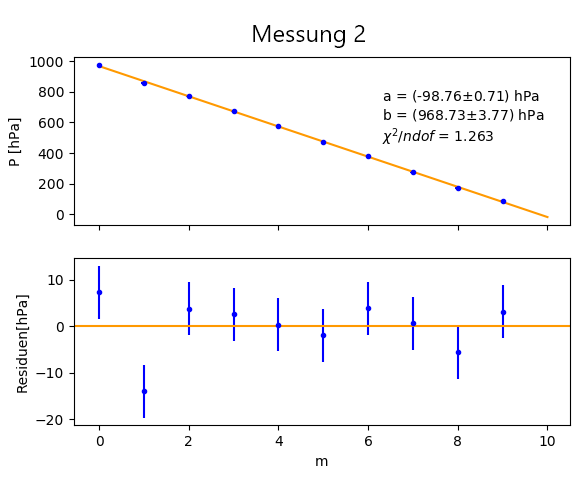
\includegraphics[scale=0.5]{Bilder/Druck_A_Var2_2.png}
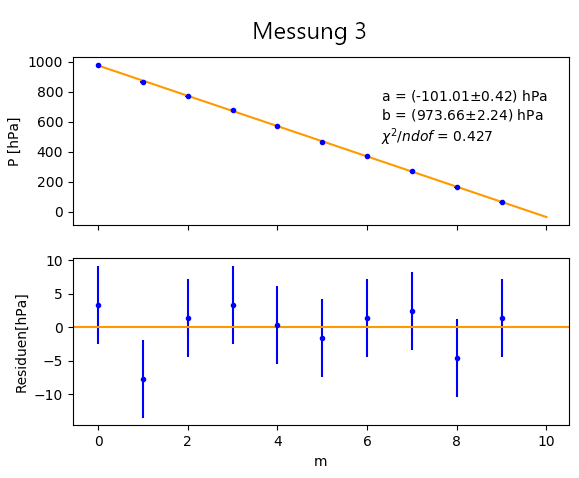
\includegraphics[scale=0.5]{Bilder/Druck_A_Var2_3.png}
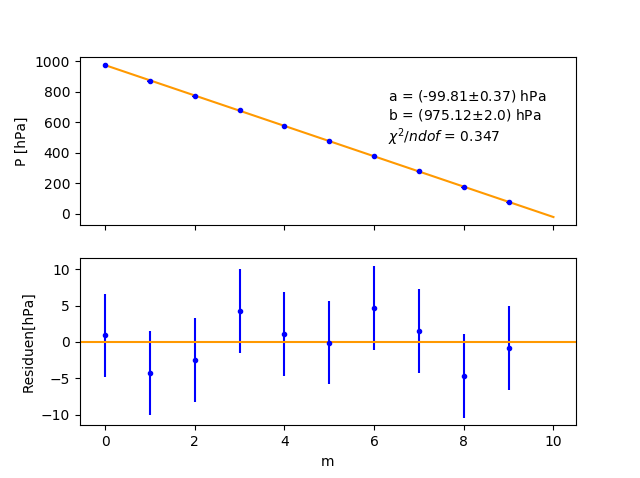
\includegraphics[scale=0.5]{Bilder/Druck_A_Var2_4.png}
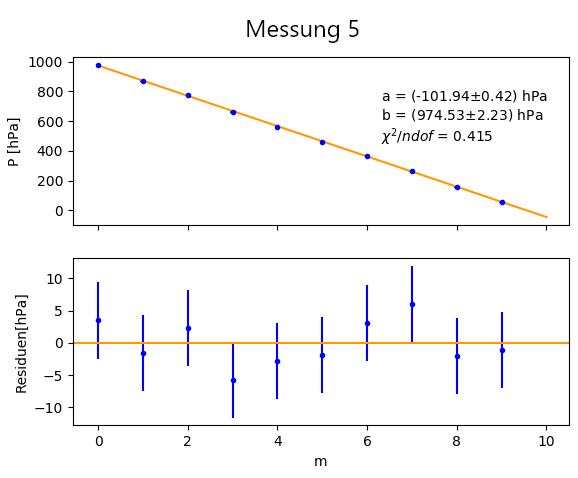
\includegraphics[scale=0.5]{Bilder/Druck_A_Var2_5.png}
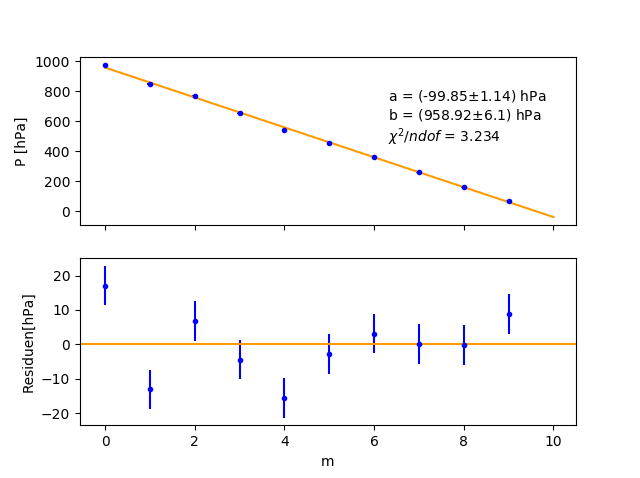
\includegraphics[scale=0.5]{Bilder/Druck_A_Var2_6.png}
\caption{Lineare Regressionen für die übgrigen Messreihen von Aufbau A}
\end{figure}

\subsubsection{Lineare Regressionen Aufbau B (TODO)}
\begin{figure}
\centering
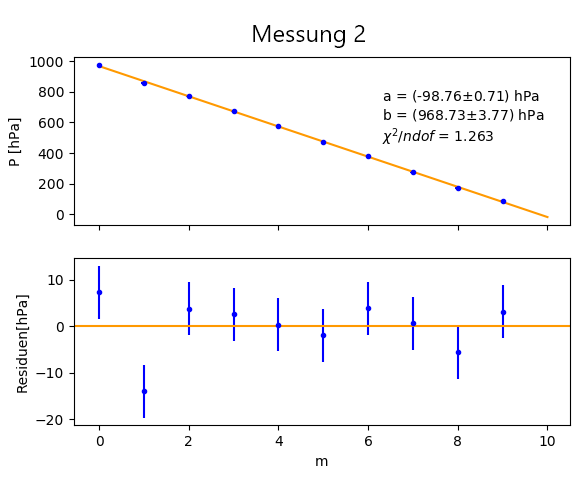
\includegraphics[scale=0.5]{Bilder/Druck_A_Var2_2.png}
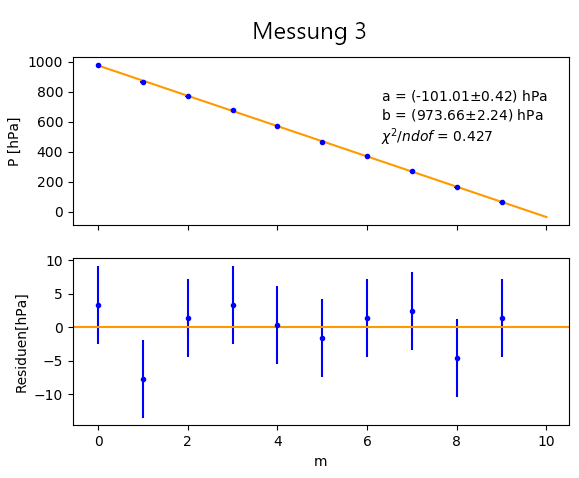
\includegraphics[scale=0.5]{Bilder/Druck_A_Var2_3.png}
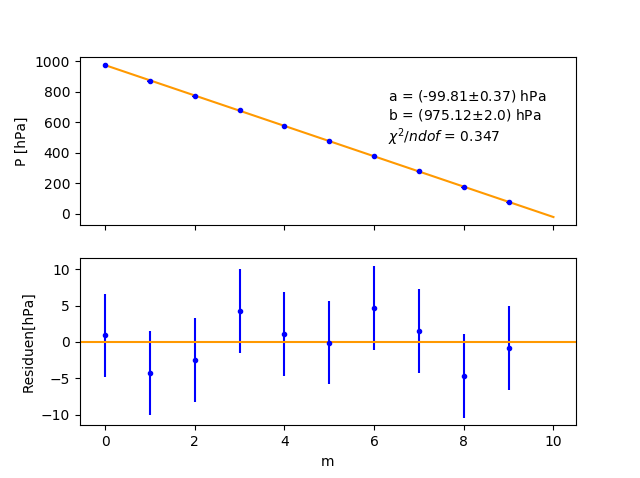
\includegraphics[scale=0.5]{Bilder/Druck_A_Var2_4.png}
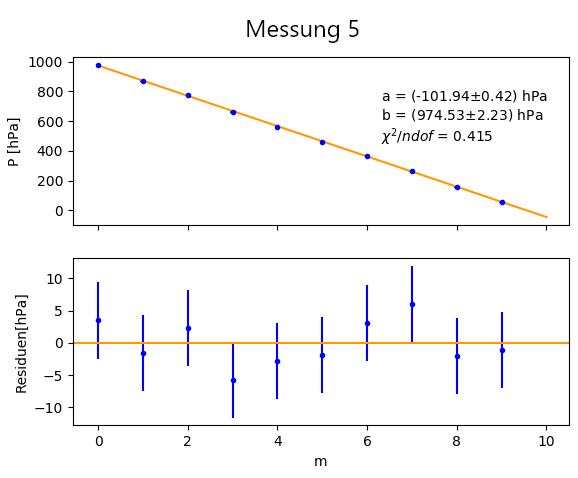
\includegraphics[scale=0.5]{Bilder/Druck_A_Var2_5.png}
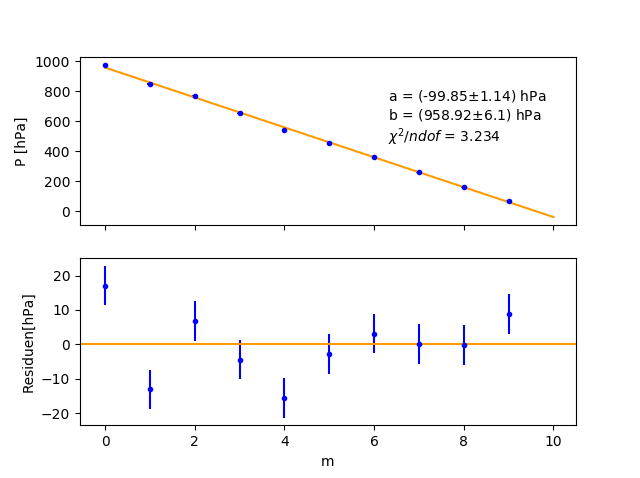
\includegraphics[scale=0.5]{Bilder/Druck_A_Var2_6.png}
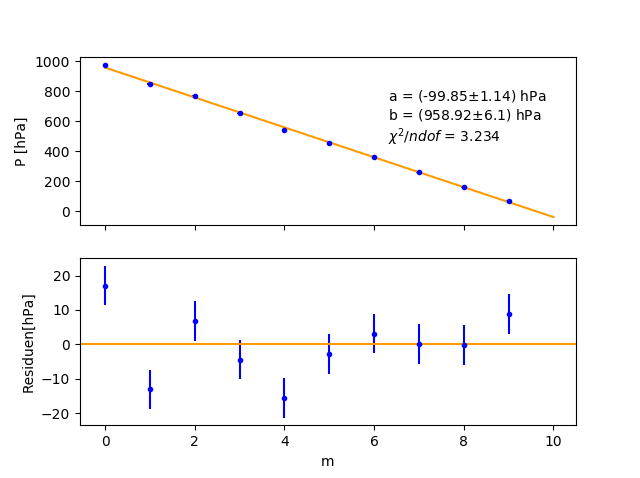
\includegraphics[scale=0.5]{Bilder/Druck_A_Var2_6.png}
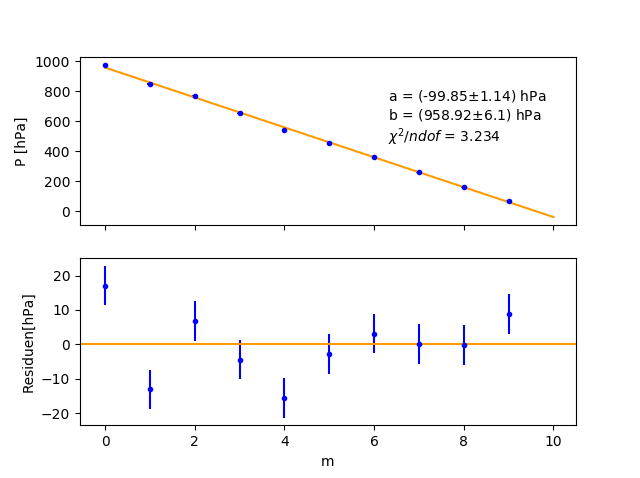
\includegraphics[scale=0.5]{Bilder/Druck_A_Var2_6.png}
\caption{Lineare Regressionen für die übgrigen Messreihen von Aufbau B}
\end{figure}

\end{document}

